\documentclass[a4paper]{article}
\usepackage[utf8]{inputenc}
\usepackage[T1]{fontenc}      
\usepackage[english]{babel} %utilisation du package français
%
%
%
\usepackage{textcomp}% améliore certains symboles de bases
\usepackage{lmodern}% remplace la police ComputerModern par LatinModern (+ mieux bien)
%
%
%
\usepackage{mathtools}% compléments à amsmath
\usepackage{amssymb,amsfonts}% symboles mathématiques supplémentaires
\usepackage{amsthm}% environnement ams-theorem
\usepackage[colorlinks,breaklinks,bookmarks,plainpages=false,unicode=true]{hyperref}%
\usepackage{todonotes} %ajouter des commentaires
%\usepackage[disable]{todonotes}%cache les commentaires
\usepackage{datetime} %ajoute la date et l'heure
%
%
\usepackage{tikz}
\usetikzlibrary{external,graphs}
\tikzexternalize[prefix=Images/]% On externalise. Les images sont stockées dans le dossier Images
\makeatletter %pour ne pas prendre en compte les todo dans l'externalisation
\renewcommand{\todo}[2][]{\tikzexternaldisable\@todo[#1]{#2}\tikzexternalenable}
\makeatother
\makeatletter %pour ne pas prendre en compte les missingfigures dans l'externalisation
\renewcommand{\missingfigure}[2][]{\tikzexternaldisable\@missingfigure[#1]{#2}\tikzexternalenable}
\makeatother

\tikzset{myloop above/.style={loop, out=130, in = 50,min distance =8mm}}
\tikzset{myloop below/.style={loop, out=-130, in = -50,min distance =8mm}}
\tikzset{blacknode/.style={shape= circle, fill = black, inner sep = 0pt, outer sep = 0pt, minimum size = 3pt,draw}}
%
\newtheorem{lem}{Lemma}[section]
\newtheorem{conjecture}[lem]{Conjecture}
\newtheorem{cor}[lem]{Corollary}
\newtheorem{prop}[lem]{Proposition}
\newtheorem{thm}[lem]{Theorem}
\theoremstyle{definition}
\newtheorem{defn}[lem]{Definition}
\newtheorem{rem}[lem]{Remark}
\theoremstyle{remark}% texte en roman
\newtheorem{exmp}[lem]{Example}
%
%
%
\DeclareMathOperator\Cayley{Cayl}
\DeclareMathOperator\Sch{Sch}
\DeclareMathOperator\stab{Stab}
\DeclareMathOperator\Ind{Ind}
%
\DeclarePairedDelimiter\abs{\lvert}{\rvert}
\newcommand*{\orbite}{\mathcal O}
\newcommand*{\field}[1]{\mathbf{#1}}
\newcommand*{\Z}{\field{Z}}
\newcommand*{\N}{\field{N}}
\newcommand{\setst}[2]{\{#1\ |\ #2\}}
\newcommand*{\powerset}[1]{\mathcal P(#1)}
\newcommand*{\powersetf}[1]{\mathcal P_{\textnormal{f}}(#1)}
\newcommand*{\powersetcof}[1]{\mathcal P_{\textnormal{cof}}(#1)}
%
%
\title{Wreath products of groups acting with bounded orbits}
\author{Paul-Henry Leemann, Grégoire Schneeberger}
\date{\today \quad \currenttime}
%
%
%
%
%
%
%
%
%
%
\begin{document}
\maketitle
%
%
%
%
%
%
%
%
%
%
\begin{abstract}

\end{abstract}
%
%
%
%
%
%
%
%
%
%
%
%
%
%
%
%%!TEX root = ends.tex
%
%
%
%
%
%
%
%
%
%
%%%%%%%%%%%%%%%%%%%%%%%%%%%%%%%%%%%%%%%%%%%%%%%%%%%%%%%%%%%%%%%%%%%%%%%%%%%
%%%%%%%%%%%%%%%%%%%%%%%%%%%%%%%%%%%%%%%%%%%%%%%%%%%%%%%%%%%%%%%%%%%%%%%%%%%
%%%%%%%%%%%%%%%%%%%%%%%    Section : Introduction    %%%%%%%%%%%%%%%%%%%%%%
%%%%%%%%%%%%%%%%%%%%%%%%%%%%%%%%%%%%%%%%%%%%%%%%%%%%%%%%%%%%%%%%%%%%%%%%%%%
%%%%%%%%%%%%%%%%%%%%%%%%%%%%%%%%%%%%%%%%%%%%%%%%%%%%%%%%%%%%%%%%%%%%%%%%%%%
\section{Introduction}
%
%
%
%
%
Property FW is a group property that is (for discrete groups) a weakening of the celebrated Kazdhan's property (T). It was introduced by Barnhill and Chatterji in \cite{Barnhill2008} and studied extensively by Cornulier in \cite{Cornulier2013}. It is a fixed point property for actions on wall spaces and hence stands between property FH (fixed points on Hilbert spaces, equivalent to property (T) for discrete groups) and property FA (fixed points on \emph{arbres}\footnote{\emph{Arbres} is the french word for trees.}), see \cite{Cornulier2013} for more details.

When working with group properties, it is natural to ask if they are stable under ``natural'' group operations. For example, one may wonder when a property is stable by subgroups, quotients, direct products or semi-direct products.
A slightly less common operation, but still of great use in geometric group theory, is the wreath product, see Definition~\ref{Def:WreathProd}.

In the context of properties defined by fixed points of actions, the first result concerning wreath products was due to Cherix, Martin and Valette and latter refined by Neuhauser and concern property (T).
%
%
\begin{thm}[\cite{Cherix2004,Neuhauser2005a}] \label{T:Wreath_prop_T}
Let $G,H$ be two discrete groups with $G$ non-trivial and $X$ a set on which $H$ acts. The wreath product $G \wr_X H$ has property (T) if and only if $G$ and $H$ have property (T) and $X$ is finite.
\end{thm}
%
%
A somewhat similar result for property FA was obtained by Cornulier and Kar in \cite{Cornulier2011}.
Cornulier also obtained partial results on wreath products and property FW in \cite{Cornulier2013}.

The aim of this note is to give an elementary proof of the analogous of Theorem~\ref{T:Wreath_prop_T} for property FW:
%
%
\begin{thm}\label{Thm:Main}
Let $G,H$ be two finitely generated groups with $G$ non-trivial and $X$ a set on which $H$ acts with finitely many orbits. The wreath product $G \wr_X H$ has property FW if and only if $G$ and $H$ have property FW and $X$ is finite.
\end{thm}
%
%
Our proof will rely on a characterization of property FW via ends of Schreier graphs \cite{Cornulier2013}, see Subsection \ref{Subsection:FW} for the relevant definitions.

At his point, the curious reader might have two questions. First, is it possible to extend Theorem \ref{Thm:Main} beyond the realms of finitely generated groups and of actions with finitely many orbits? And secondly, is there a link between Theorems \ref{T:Wreath_prop_T} and \ref{Thm:Main}?
In both cases, the answer is yes.
This is the subject of the forthcoming and more technical \cite{LS2021}, which gives an unified proof of Theorems \ref{T:Wreath_prop_T} and \ref{Thm:Main} as well as of similar results for the Bergman property and more.
%
%
%
%
\paragraph{Organization of the paper}
The next section contains all the definitions as well as some examples, while Section \ref{Section:Proof} is devoted to the proof of Theorem~\ref{Thm:Main} and some related results.
%
%
%
%\todo[inline]{Mettre ici les remerciements. Tu dois possiblement remercier la NSF. J'ai mis Alain en remerciement, je ne sais pas ce que tu en penses et si tu veux être plus spécifique.}
\paragraph{Acknowledgment}
The authors are thankful to A. Valette for comments on a previous version of this note.
The first author was supported by NSF Grant No. 200021\textunderscore188578. The second author thanks Tatiana Nagnibeda for her comments and the SNF for its support.
%
%
%
%\todo[inline]{J'ai mis en commentaire la partie sur les actions essentielles ne sachant pas comment l'introduire. Je pense que si on veut la garder, le mieux est de la mettre un peu en apparté soit à la fin de l'intro soit à la fin de l'article. Cela permet de garder quelque chose de simple et d'auto-contenu pour le reste.}

%An action of a group on a CAT(0) cube complex is \emph{essential} if all the orbits of vertices are unbounded and the action is transitive on the set of hyperplanes.
%\begin{cor}
%Let $G,H$ be two discrete groups and $X$ a set on which $H$ acts transitively. If there exists an essential action of $G$ or $H$ on a CAT(0) cube complex  or if $X$ is infinite, then there exists an essential action of $G \wr_X H$ on a CAT(0) cube complex. 
%\end{cor}
%%!TEX root = ends.tex
%
%
%
%
%
%
%
%
%
%
%%%%%%%%%%%%%%%%%%%%%%%%%%%%%%%%%%%%%%%%%%%%%%%%%%%%%%%%%%%%%%%%%%%%%%%%%%%
%%%%%%%%%%%%%%%%%%%%%%%%%%%%%%%%%%%%%%%%%%%%%%%%%%%%%%%%%%%%%%%%%%%%%%%%%%%
%%%%%%%%%%%%%%%%%    Section : Definitions and examples    %%%%%%%%%%%%%%%%
%%%%%%%%%%%%%%%%%%%%%%%%%%%%%%%%%%%%%%%%%%%%%%%%%%%%%%%%%%%%%%%%%%%%%%%%%%%
%%%%%%%%%%%%%%%%%%%%%%%%%%%%%%%%%%%%%%%%%%%%%%%%%%%%%%%%%%%%%%%%%%%%%%%%%%%
\section{Definitions and examples}
This section contains all the definitions, as well as some useful preliminaries facts and some examples.
All the results cited in this section are standard.
% and can be found in any good book about geometric group theory, see for example~\cite{DelaHarpe2000}.\todo{Peut-être retravailler l'intro.} 
%
%
%
%
%
%
%
%
%
%
%%%%%%%%%%%%%%%%%%%%%%%%%%%%%%%%%%%%%%%%%%%%%%%%%%%%%%%%%%%%%%%%%%%%%%%%%%%
%%%%%%%%%%%%%%%%%%%%%%%%%%%%%%%%%%%%%%%%%%%%%%%%%%%%%%%%%%%%%%%%%%%%%%%%%%%
%%%%%%%%    Subsection : Ends of Schreier graphs and property FW    %%%%%%%
%%%%%%%%%%%%%%%%%%%%%%%%%%%%%%%%%%%%%%%%%%%%%%%%%%%%%%%%%%%%%%%%%%%%%%%%%%%
%%%%%%%%%%%%%%%%%%%%%%%%%%%%%%%%%%%%%%%%%%%%%%%%%%%%%%%%%%%%%%%%%%%%%%%%%%%
\subsection{Ends of Schreier graphs and property FW}
\label{Subsection:FW}
%
%
%
%
%
In what follows, we will always assume that generating sets of groups are \emph{symmetric}, that is we will look at $S\subset G$ such that $s\in S$ if and only if $s^{-1}\in S$.
Our graphs will be undirected and we will sometimes identify  graph with its vertex set.
%
%
\begin{defn}
Let $G$ be a group, $H$ a subgroup of $G$ and $S$ a symmetric generating set. The \emph{(left) Schreier graph} $\Sch(G,H;S)$ is the graph with vertices the left cosets $gH=\setst{gh}{h\in H}$ and with an edge between $gH$ and $sgH$ for every $s$ in $S$.
\end{defn}
%
%
Observe that with the above definition, a Schreier graph may have loops as well as multiple edges. Moreover, in $\Sch(G,H;S)$ every vertex has degree $\abs S$.

If $X$ is a set with a left action $G\curvearrowright X$ and $S$ is a symmetric generating set for $G$, the corresponding (left) \emph{orbital graph} $\Sch_{\mathcal O}(G,X;S)$ is the graph with vertex set $X$ and with an edge between $x$ and $y$ for every $s$ in $S$ such that $s.x=y$.
As the notation suggest, these two definitions are the two faces of the same coin. Indeed, we have $\Sch(G,H;S)=\Sch_{\mathcal O}(G,G/H;S)$ for the  action by left multiplication of $G$ on $G/H$, while   for every $x\in X$, the graph $\Sch(G,\stab_G(x);S)$ is equal to the connected component of $x$ in $\Sch_{\mathcal O}(G,X;S)$.

Schreier graphs are generalizations of the well-known \emph{Cayley graphs}, with $\Cayley(G;S)=\Sch(G,\{1\};S)$.

If $S$ and $T$ are two generating sets of $G$, the graphs $\Sch(G,H;S)$ and $\Sch(G,H;T)$ need not to be isomorphic. However, if both $S$ and $T$ are finite, then $\Sch(G,H;S)$ and $\Sch(G,H;T)$ are quasi-isometric, see \cite[IV.B.21.iii]{DelaHarpe2000} for a proof and Figure~\ref{Figure:CayleyOfZ} for an example. The only fact we will use about quasi-isometries is that they preserve ``large-scale properties'' of the graph, as for examples the number of ends.
Observe that the requirement that both $S$ and $T$ are finite is crucial for the existence of a quasi-isometry between the corresponding Schreier graphs. Indeed, for every group  $\Cayley(G;G\setminus\{1\})=\Sch(G,\{1\};G\setminus\{1\})$ is always a complete graph on $\abs{G}$ vertices, in particular  $\Cayley(\Z;\{1\})$ and $\Cayley(\Z;\Z\setminus\{0\})$ are not quasi-isometric.
%
%
\begin{figure}[htbp]\centering
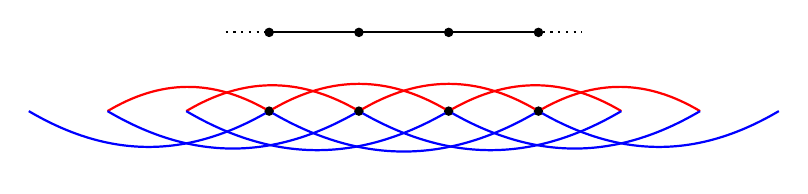
\begin{tikzpicture}[node distance=1.14cm,every node/.style=blacknode]
\node (0){} ;
\coordinate[left =0.5cm of 0] (a) ;
\node (1)[right of=0]{} ;
\node (2)[right of=1]{} ;
\node (3)[right of=2]{} ;
\coordinate[right =0.5cm of 3] (b) ;
\graph[edge={thick}]{(a)--[dotted](0)--(1)--(2)--(3)--[dotted](b)} ;

\begin{scope}[yshift=-1cm]
\node (0){} ;
%\coordinate[left =0.5cm of 0] (a) ;
\coordinate[left =1cm of 0] (-1) ;
\coordinate[left =2cm of 0] (-2) ;
\coordinate[left =3cm of 0] (-3) ;
\node (1)[right of=0]{} ;
\node (2)[right of=1]{} ;
\node (3)[right of=2]{} ;
%\node (4)[right of=3]{} ;
%\coordinate[right =0.5cm of 4] (b) ;
\coordinate[right =1cm of 3] (4) ;
\coordinate[right =2cm of 3] (5) ;
\coordinate[right =3cm of 3] (6) ;
\graph[edge={thick}]{(-2)--[bend left,red](0)--[bend left,red](2)--[bend left,red](4), (-1)--[bend left,red](1)--[bend left,red](3)--[bend left,red](5) } ;
\graph[edge={thick}]{(-3)--[bend right,blue](0)--[bend right,blue](3)--[bend right,blue](6), (-2)--[bend right,blue](1)--[bend right,blue](4),(-1)--[bend right,blue](2)--[bend right,blue](5)} ;
\end{scope}
\end{tikzpicture}
\caption{Fragments of two Cayley graphs of $\Z$ ($2$ ends), for the standard generating set $\{\pm1\}$ and for the generating set $\{\textcolor{red}{\pm2},\textcolor{blue}{\pm3}\}$.}
\label{Figure:CayleyOfZ}
\end{figure}
\begin{figure}[htbp]\centering
\begin{subfigure}{0.5\textwidth}
\centering
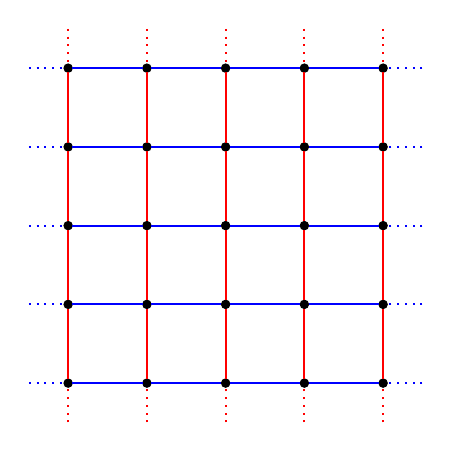
\begin{tikzpicture}
\foreach \i in {1,...,25}
{
        \pgfmathtruncatemacro{\y}{(\i - 1) / 5} ;
        \pgfmathtruncatemacro{\x}{\i - 5 * \y} ;
        \pgfmathtruncatemacro{\label}{\x + 5 * (4 - \y)} ;
        \node[blacknode] (\label) at (1*\x,-1*\y) {} ;
}
\foreach \i in {1,...,5}{
	\draw[thick, blue,dotted] (0.5,-\i+1)--(0.95,-\i+1) ;
	\draw[thick, blue,dotted] (5.5,-\i+1)--(5.05,-\i+1) ;
	\draw[thick, red,dotted] (\i,-4.5)--(\i,-4.05) ;
	\draw[thick, red,dotted] (\i,0.5)--(\i,0.05) ;
	\foreach \j in {0,...,3}{
		\pgfmathtruncatemacro{\x}{1+5*(\i-1)+\j} ;
		\pgfmathtruncatemacro{\y}{\x+1} ;
		\draw[thick, blue](\x)--(\y) ;
		\pgfmathtruncatemacro{\zz}{\i+5*\j} ;
		\pgfmathtruncatemacro{\t}{\zz+5} ;
		\draw[thick, red] (\zz)--(\t) ;
	}
}
\end{tikzpicture}
%\caption{Lorem ipsum}
\end{subfigure}%
\begin{subfigure}{0.5\textwidth}
\centering
\scalebox{0.8}{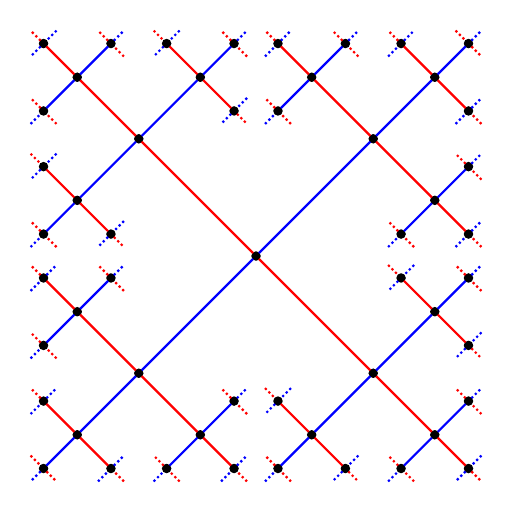
\begin{tikzpicture}[every node/.style=blacknode]
\useasboundingbox (-2.9,-2.9) rectangle (2.9,2.9);
\rotatebox{45}{
\node (0){};
\foreach \i/\j in {E/right,W/left}{
\node (\i)[\j = 2cm of 0]{} ;
\node (\i\i)[\j = 1cm of \i]{} ;
	\node (\i\i N)[above = 0.5cm of \i\i]{} ;
		\coordinate[above =0.18cm of \i\i N] (\i\i NN) ;
		\coordinate[right =0.18cm of \i\i N] (\i\i NE) ;
		\coordinate[left =0.18cm of \i\i N] (\i\i NW) ;
	\node (\i\i S)[below = 0.5cm of \i\i]{} ;
		\coordinate[below =0.18cm of \i\i S] (\i\i SS) ;
		\coordinate[right =0.18cm of \i\i S] (\i\i SE) ;
		\coordinate[left =0.18cm of \i\i S] (\i\i SW) ;
	\node (\i\i\i)[\j = 0.5cm of \i\i]{} ;
		\coordinate[\j =0.18cm of \i\i\i] (\i\i\i\i) ;
		\coordinate[above =0.18cm of \i\i\i] (\i\i\i N) ;
		\coordinate[below =0.18cm of \i\i\i] (\i\i\i S) ;
\node (\i N)[above = 1cm of \i ]{} ;
	\node (\i NN)[above = 0.5cm of \i N]{} ;
		\coordinate[above =0.18cm of \i NN] (\i NNN) ;
		\coordinate[right =0.18cm of \i NN] (\i NNE) ;
		\coordinate[left =0.18cm of \i NN] (\i NNW) ;
	\node (\i NW)[left = 0.5cm of \i N]{} ;
		\coordinate[above =0.18cm of \i NW] (\i NWN) ;
		\coordinate[below =0.18cm of \i NW] (\i NWS) ;
		\coordinate[left =0.18cm of \i NW] (\i NWW) ;
	\node (\i NE)[right = 0.5cm of \i N]{} ;
		\coordinate[above =0.18cm of \i NE] (\i NEN) ;
		\coordinate[below =0.18cm of \i NE] (\i NES) ;
		\coordinate[right =0.18cm of \i NE] (\i NEE) ;
\node (\i S)[below = 1cm of \i ]{} ;
	\node (\i SS)[below = 0.5cm of \i S]{} ;
		\coordinate[below =0.18cm of \i SS] (\i SSS) ;
		\coordinate[right =0.18cm of \i SS] (\i SSE) ;
		\coordinate[left =0.18cm of \i SS] (\i SSW) ;
	\node (\i SW)[left = 0.5cm of \i S]{} ;
		\coordinate[above =0.18cm of \i SW] (\i SWN) ;
		\coordinate[below =0.18cm of \i SW] (\i SWS) ;
		\coordinate[left =0.18cm of \i SW] (\i SWW) ;
	\node (\i SE)[right = 0.5cm of \i S]{} ;
		\coordinate[above =0.18cm of \i SE] (\i SEN) ;
		\coordinate[below =0.18cm of \i SE] (\i SES) ;
		\coordinate[right =0.18cm of \i SE] (\i SEE) ;
\graph[edge={thick,color=blue}]{
(0)--(\i )--(\i\i)--(\i\i\i)--[densely dotted](\i\i\i\i),
(\i SWW)--[densely dotted](\i SW)--(\i S)--(\i SE)--[densely dotted](\i SEE),
(\i NWW)--[densely dotted](\i NW)--(\i N)--(\i NE)--[densely dotted](\i NEE),
(\i NNW)--[densely dotted](\i NN)--[densely dotted](\i NNE),
(\i SSW)--[densely dotted](\i SS)--[densely dotted](\i SSE),
(\i\i NW)--[densely dotted](\i\i N)--[densely dotted](\i\i NE),
(\i\i SW)--[densely dotted](\i\i S)--[densely dotted](\i\i SE)
};
\graph[edge={thick,color=red}]{
	(\i SSS)--[densely dotted](\i SS)--(\i S)--(\i)--(\i N)--(\i NN)--[densely dotted](\i NNN),
	(\i\i SS)--[densely dotted](\i\i S)--(\i\i)--(\i\i N)--[densely dotted](\i\i NN),
	(\i\i\i N)--[densely dotted](\i\i\i)--[densely dotted](\i\i\i S),
	(\i NES)--[densely dotted](\i NE)--[densely dotted](\i NEN),
	(\i SES)--[densely dotted](\i SE)--[densely dotted](\i SEN),
	(\i NWS)--[densely dotted](\i NW)--[densely dotted](\i NWN),
	(\i SWS)--[densely dotted](\i SW)--[densely dotted](\i SWN)
};
}
\foreach \i/\j in {N/above,S/below}{
\node (\i)[\j = 2cm of 0]{} ;
\node (\i\i)[\j = 1cm of \i]{} ;
	\node (\i\i W)[left = 0.5cm of \i\i]{} ;
		\coordinate[above =0.18cm of \i\i W] (\i\i WN) ;
		\coordinate[below =0.18cm of \i\i W] (\i\i WS) ;
		\coordinate[left =0.18cm of \i\i W] (\i\i WW) ;	
	\node (\i\i E)[right = 0.5cm of \i\i]{} ;
		\coordinate[above =0.18cm of \i\i E] (\i\i EN) ;
		\coordinate[below =0.18cm of \i\i E] (\i\i ES) ;
		\coordinate[right =0.18cm of \i\i E] (\i\i EE) ;
	\node (\i\i\i)[\j = 0.5cm of \i\i]{} ;
		\coordinate[\j =0.18cm of \i\i\i] (\i\i\i\i) ;
		\coordinate[right =0.18cm of \i\i\i] (\i\i\i E) ;
		\coordinate[left =0.18cm of \i\i\i] (\i\i\i W) ;
\node (\i E)[right = 1cm of \i ]{} ;
	\node (\i EE)[right = 0.5cm of \i E]{} ;
		\coordinate[above =0.18cm of \i EE] (\i EEN) ;
		\coordinate[below =0.18cm of \i EE] (\i EES) ;
		\coordinate[right =0.18cm of \i EE] (\i EEE) ;
	\node (\i ES)[below = 0.5cm of \i E]{} ;
		\coordinate[below =0.18cm of \i ES] (\i ESS) ;
		\coordinate[left =0.18cm of \i ES] (\i ESE) ;
		\coordinate[right =0.18cm of \i ES] (\i ESW) ;
	\node (\i EN)[above = 0.5cm of \i E]{} ;
		\coordinate[above =0.18cm of \i EN] (\i ENN) ;
		\coordinate[left =0.18cm of \i EN] (\i ENE) ;
		\coordinate[right =0.18cm of \i EN] (\i ENW) ;
\node (\i W)[left = 1cm of \i ]{} ;
	\node (\i WS)[below = 0.5cm of \i W]{} ;
		\coordinate[below =0.18cm of \i WS] (\i WSS) ;
		\coordinate[left =0.18cm of \i WS] (\i WSE) ;
		\coordinate[right =0.18cm of \i WS] (\i WSW) ;
	\node (\i WN)[above = 0.5cm of \i W]{} ;
		\coordinate[above =0.18cm of \i WN] (\i WNN) ;
		\coordinate[left =0.18cm of \i WN] (\i WNE) ;
		\coordinate[right =0.18cm of \i WN] (\i WNW) ;
	\node (\i WW)[left = 0.5cm of \i W]{} ;
		\coordinate[above =0.18cm of \i WW] (\i WWN) ;
		\coordinate[below =0.18cm of \i WW] (\i WWS) ;
		\coordinate[left =0.18cm of \i WW] (\i WWW) ;
\graph[edge={thick,color=red}]{
	(0)--(\i )--(\i\i)--(\i\i\i)--[densely dotted](\i\i\i\i),
	(\i ENN)--[densely dotted](\i EN)--(\i E)--(\i ES)--[densely dotted](\i ESS),
	(\i WNN)--[densely dotted](\i WN)--(\i W)--(\i WS)--[densely dotted](\i WSS),
	(\i EES)--[densely dotted](\i EE)--[densely dotted](\i EEN),
	(\i WWS)--[densely dotted](\i WW)--[densely dotted](\i WWN),
	(\i\i ES)--[densely dotted](\i\i E)--[densely dotted](\i\i EN),
	(\i\i WS)--[densely dotted](\i\i W)--[densely dotted](\i\i WN)};
\graph[edge={thick,color=blue}]{
	(\i WWW)--[densely dotted](\i WW)--(\i W)--(\i)--(\i E)--(\i EE)--[densely dotted](\i EEE),
	(\i\i WW)--[densely dotted](\i\i W)--(\i\i)--(\i\i E)--[densely dotted](\i\i EE),
	(\i ENW)--[densely dotted](\i EN)--[densely dotted](\i ENE),
	(\i ESW)--[densely dotted](\i ES)--[densely dotted](\i ESE),
	(\i WNW)--[densely dotted](\i WN)--[densely dotted](\i WNE),
	(\i WSW)--[densely dotted](\i WS)--[densely dotted](\i WSE),
	(\i\i\i E)--[densely dotted](\i\i\i)--[densely dotted](\i\i\i W)};
}
}
\end{tikzpicture}}
%\caption{Lorem ipsum}
\end{subfigure}
\caption{Fragments of the Cayley graphs of $\Z^2$ ($1$ end) on the left and of $F_2$ (infinitely many ends) on the right; with standard generating sets.}
\label{Figure:CayleyOfZ2}
\end{figure}
\begin{figure}[htbp]\centering
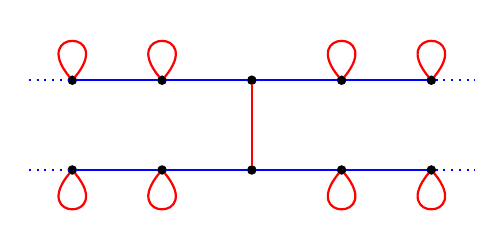
\begin{tikzpicture}[node distance=1.14cm,every node/.style=blacknode]
\node (00){} ;
\coordinate[left =0.5cm of 00] (0a) ;
\node (01)[right of=00]{} ;
\node (02)[right of=01]{} ;
\node (03)[right of=02]{} ;
\node (04)[right of=03]{} ;
\coordinate[right =0.5cm of 04] (0b) ;
\node (10)[above of=00]{} ;
\coordinate[left =0.5cm of 10] (1a) ;
\node (11)[above of=01]{} ;
\node (12)[above of=02]{} ;
\node (13)[above of=03]{} ;
\node (14)[above of=04]{} ;
\coordinate[right =0.5cm of 14] (1b) ;
\graph[edge={thick,color=blue}]{(0a)--[dotted](00)--(01)--(02)--(03)--(04)--[dotted](0b)} ;
\graph[edge={thick,color=blue}]{(1a)--[dotted](10)--(11)--(12)--(13)--(14)--[dotted](1b)} ;
\graph[edge={thick,color=red}]{(02)--(12)} ;
\foreach \i in {0,1,3,4}{
\draw [thick,color=red] (0\i) to [myloop below] (0\i) ;
\draw [thick,color=red] (1\i) to [myloop above] (1\i) ;
}
%\begin{scope}[yshift=-1cm]
%\node (0){} ;
%%\coordinate[left =0.5cm of 0] (a) ;
%\coordinate[left =1cm of 0] (-1) ;
%\coordinate[left =2cm of 0] (-2) ;
%\coordinate[left =3cm of 0] (-3) ;
%\node (1)[right of=0]{} ;
%\node (2)[right of=1]{} ;
%\node (3)[right of=2]{} ;
%%\node (4)[right of=3]{} ;
%%\coordinate[right =0.5cm of 4] (b) ;
%\coordinate[right =1cm of 3] (4) ;
%\coordinate[right =2cm of 3] (5) ;
%\coordinate[right =3cm of 3] (6) ;
%\graph[edge={thick}]{(-2)--[bend left,red](0)--[bend left,red](2)--[bend left,red](4), (-1)--[bend left,red](1)--[bend left,red](3)--[bend left,red](5) } ;
%\graph[edge={thick}]{(-3)--[bend right,blue](0)--[bend right,blue](3)--[bend right,blue](6), (-2)--[bend right,blue](1)--[bend right,blue](4),(-1)--[bend right,blue](2)--[bend right,blue](5)} ;
%\end{scope}
\end{tikzpicture}
\caption{A fragment of a Schreier graph (with $4$ ends) of the free group $F_2=\langle \textcolor{red}{x^{\pm1}},\textcolor{blue}{y^{\pm1}}\rangle$.}
\label{Figure:SchreierOfF2}
\end{figure}
%
%
Let $\Gamma$ be a graph and $K$ a finite subset of vertices. The graph $\Gamma\setminus K$ is the subgraph of $\Gamma$ obtained by deleting all vertices in $K$ and all edges adjacent to them. This graph is not necessarily connected.
\begin{defn}\label{Def:Ends}
Let $\Gamma$ be a graph. The \emph{number of ends} of $\Gamma$ is the supremum, taken over all finite $K$, of the number of infinite connected components of $\Gamma\setminus K$.
\end{defn}
There exists other characterization of the number of ends in graphs, %notably in terms of equivalence classes of rays,
see \cite{MR1967888} and the references therein, but Definition \ref{Def:Ends} is the one that best suits our purpose.
%The interested reader may refer to \cite{MR1967888} and the references therein for an extended treatment of the 
A locally finite graph (i.e. such that every vertex has finite degree) is finite if and only if it has $0$ ends.
%The graphs of the Figures~\ref{Figure:CayleyOfZ} and \ref{Figure:CayleyOfZ2} have respectively 2 ends and 1 end. 

An important fact about the number of ends of a graph, is that it is an invariant of quasi-isometry, see \cite{MR1213151}. In particular, if $G$ is a finitely generated group it is possible to speak about the number of ends of the Schreier graph $\Sch(G,H;S)$ without specifying a particular finite generating set $S$.
By a celebrated result of Stallings \cite{Stallings1971}, the number of ends of a Cayley graph of a finitely generated group can only be $0$, $1$, $2$ or infinite (in which case it is uncountable), see Figures~\ref{Figure:CayleyOfZ} and \ref{Figure:CayleyOfZ2} for examples.
On the other hand, Schreier graphs may have any number of ends in $\mathbf N\cup\{\infty\}$, see Figure~\ref{Figure:SchreierOfF2} for an example of a graph with $4$ ends.
%While the number of ends of Cayley graphs of finitely generated groups can only be $0$, $1$, $2$ or infinite (in which case it is uncountable) \cite[Theorem 11.27]{Stallings1971}, Schreier graphs may have any number of ends in $\mathbf N\cup\{\infty\}$, see Figure~\ref{Figure:SchreierOfF2} for an example of a graph with another number of ends.
In fact, every regular graph of even degree is isomorphic to a Schreier graph, \cite{MR0450121,MR1358635}. 

We are now finally able to introduce property FW. The following characterization is due to Cornulier \cite{Cornulier2013}.
%
%
\begin{defn}
A finitely generated group $G$ has \emph{property FW} if all its Schreier graphs have at most one end.
\end{defn}
%
%
It directly follows from the definition that all finite groups have property FW, but that $\Z$ does not have it.
In fact, if $G$ is a finitely generated group with an homomorphism onto $\Z$, then it does not have FW. Indeed, in this case $G\cong H\rtimes \Z$  for some $H$ and the Schreier graph $\Sch(G,H;S)$ will be isomorphic to a Cayley graph of $\Z\cong G/H$ and hence has $2$ ends.

Property FW admits many distinct characterizations that allow to define it for groups that are non-necessarily finitely generated and even for topological groups. We refer the reader to \cite{Cornulier2013} for a survey of these characterizations.
%
%
%
%
%
%
%
%
%
%
%%%%%%%%%%%%%%%%%%%%%%%%%%%%%%%%%%%%%%%%%%%%%%%%%%%%%%%%%%%%%%%%%%%%%%%%%%%
%%%%%%%%%%%%%%%%%%%%%%%%%%%%%%%%%%%%%%%%%%%%%%%%%%%%%%%%%%%%%%%%%%%%%%%%%%%
%%%%%%%%%%%%%%%%%%%%    Subsection : Wreath products    %%%%%%%%%%%%%%%%%%%
%%%%%%%%%%%%%%%%%%%%%%%%%%%%%%%%%%%%%%%%%%%%%%%%%%%%%%%%%%%%%%%%%%%%%%%%%%%
%%%%%%%%%%%%%%%%%%%%%%%%%%%%%%%%%%%%%%%%%%%%%%%%%%%%%%%%%%%%%%%%%%%%%%%%%%%
\subsection{Wreath products}
%
%
%
%
%
Let $X$ be a set and $G$ a group. We view 
$\bigoplus_XG$ as the set of functions from $X$ to $G$ with finite support:
\[
	\bigoplus_XG=\setst{\varphi\colon X\to G}{\varphi(x)=1 \textnormal{ for all but finitely many }x}.
\]
This is naturally a group, where multiplication is taken componentwise.

If $H$ is a group acting on $X$, then it naturally acts on $\bigoplus_XG$
by $(h.\varphi)(x)=\varphi(h^{-1}.x)$.
This leads to the following definition
\begin{defn}\label{Def:WreathProd}
Let $G$ and $H$ be groups and $X$ be a set on which $H$ acts.
The \emph{(retricted) wreath product} $G\wr_XH$ is the group $(\bigoplus_XG)\rtimes H$.
\end{defn}
A prominent  source of examples of wreath products are the ones of the form $G\wr_HH$, where $H$ acts on itself by left multiplication.
In particular, the group $(\Z/2\Z)\wr_\Z\Z$ has become well-known under the name of the \emph{lamplighter group}.
Another (trivial) examples of wreath products are direct products $G\times H$ which corresponds to wreath products over a singleton $G\wr_{\{*\}}H$.

Let $S$ be a generating set of $G$ and $T$ a generating set of $H$.
Suppose that $H$ acts transitively on $X$ and let $x\in X$ be any point.
Finally, let $\delta_x^s$ be the element of $\bigoplus_XG$ defined by $\delta_x^s(x)=s$ and $\delta_x^s(y)=1_G$ if $y\neq x$ and let $\mathbf 1$ be the constant function with value $1$.
It is then standard that 
\[
	\setst{(\delta_x^s,1_H)}{s \in S} \cup \setst{(\mathbf 1,t}{t \in T}
\]
is a generating set for $G\wr_XH$.

On the other hand, it follows from the definition of the wreath product that we have
\[
	G\wr_XH\cong\bigoplus_{Y\textnormal{ is an $H$-orbit}}\bigl(G\wr_YH\bigr).
\]
We hence obtain
%
%
\begin{lem}
The group $G\wr_XH$ is finitely generated if and only if both $G$ and $H$ are finitely generated and $H$ acts on $X$ with finitely many orbits.
\end{lem}
%
%
Using the above lemma, we could reformulate Theorem~\ref{Thm:Main} in the following way:
%
%
\begin{prop}
Let $G$, $H$ be two groups with $G$ non-trivial and $X$ a set on which $H$ acts. Suppose that all three of $G$, $H$ and $G\wr_XH$ are finitely generated. Then the wreath product $G\wr_XH$ has property FW if and only if $G$ and $H$ have property FW and $X$ is finite.
\end{prop}
%!TEX root = Median.tex
\label{Section:Median}
In this section, we will investigate property FW via the action of groups on median graphs.
In order to ease readability, we will always assume our connected graphs to be non-empty.\footnote{This is coherent with the definition that a connected graph is a graph with exactly one connected component.}

For $u$ and $v$ two vertices of a connected graph $\mathcal G$, we define the total interval $[u,v]$ as the set of vertices that lie on some shortest path between $u$ and $v$.
A connected graph $\mathcal G$ is \emph{median} if for any three vertices $u$, $v$, $w$, the intersection $[u,v]\cap[v,w]\cap[u,w]$ consists of a unique vertex, denoted $m(u,v,w)$.
A graph is \emph{median} if each of its connected components is median.

Recall that a group $G$ has property FW if and only if every $G$ action on a connected median graph has bounded orbits.

\todo[inline]{Dire quelque part qu'un groupe $G$ est non-trivial ssi tout action sur un espace métrique (resp, un Hilbert, un arbre, un graphe médian connexe, un espace ultra-métrique) est uniformément bornée.

Pour un Hilbert (et donc un espace métrique), il suffit de prendre $l^2(G)$ est de regarder l'orbite de $n\cdot \delta_g$ qui a diamètre $n\sqrt2$. Pour un arbre (et donc graphe médian connexe), on prend une racine $r$ sur laquelle on colle un rayon infini pour chaque $g\in G$. On obtient un arbre $T$ sur lequel $G$ agit par permutations des rayons. Les orbites sont les $\mathcal L_n=\setst{v}{\textnormal{à distance $n$ de la racine}}$ qui ont diamètre $2n$. Finalement, on peut mettre une ultradistance sur les sommets de $T$ par $d(x,y)=\max(\mathcal L(x),\mathcal L(y),)$. Les orbites sont toujours les $\mathcal L_n$ avec diamètre $n$.}

We begin this section by proving a series of results that will be generalized to a broader context in Section~\ref{Section:Generalizations}.
The following easy lemma is folklore, and we provide a proof of it only for the sake of completeness.
\begin{lem}\label{Lemma:Subgroup}
Let $G$ be a group and $H$ be a finite index subgroup.
If $H$ has property FW, then so does~$G$.
\end{lem}
\begin{proof}
Suppose that $G$ does not have FW and let $X$ be a connected median graph on which $G$ acts with an unbounded orbit $\orbite$.
Then $H$ acts on $X$ and $\orbite$ is a union of at most $[G:H]$ orbits. This directly implies that $H$ has an unbounded orbit and therefore does not have FW.
\end{proof}

We also have the following lemma on semi-direct products:
\begin{lem}\label{Lemma:Semidirect}
Let $G=N\rtimes H$ be a semidirect product. Then
\begin{enumerate}
\item
If $G$ has property FW, then so does $H$.
\item
If both $N$ and $H$ have property FW, then $G$ also has property FW.
\end{enumerate}
\end{lem}
\begin{proof}
Suppose that $G$ has FW and let $X$ be a non-empty connected median graph on which $H$ acts.
Then $G$ acts on $X$ by $g.x\coloneqq h.x$ where $g=nh$ with $n\in N$ and $h\in H$.
By assumption, the action of $G$ on $X$ has bounded orbits and so does the action of $H$.

On the other hand, suppose that $N$ and $H$ have FW and let $X$ be a non-empty connected median graph on which $G$ acts.
Then both $N$ and $H$ acts on $X$ with bounded orbits.
Let $x$ be an element of $X$, $d_1$ the diameter of $H.x$ and $d_2$ the diameter of $N.x$.
Since $G$ acts by isometries, for every $h$ in $H$ the set $N.(h.x)=Nh.x=hN.x=h.(N.x)$ has also diameter $d_2$.
Therefore, every element of $G.x=NH.x$ is at distance at most $d_1+d_2$ of $x$, which implies that the orbit $G.x$ is bounded. %, with diameter at most $d_1+2\cdot d_2$.
\end{proof}
Multiple applications of Lemma~\ref{Lemma:Semidirect} give us
\begin{cor}\label{Cor:Wreath}
Let $G\wr_X H$ be the wreath product of $G$ and $H\curvearrowright X$.
Then
\begin{enumerate}
\item
If $G\wr_X H$ has property FW, then so does $H$.
\item
If $X$ is finite and both $G$ and $H$ have property FW, then $G\wr_X H$ has property FW.
\end{enumerate}
\end{cor}







We now turn our attention on results that will rely more on the median structure.

Trees are the simplest examples of median graphs and a simple verification shows that if $X$ and $Y$ are both (connected) median graphs, then their cartesian product is also a (connected) median graph.
On the other hand, the following example will be fundamental for us.
%
%
\begin{exmp}\label{Ex:MainMedian}
Let $X$ be a set and let  $\powerset{X}=2^X$ be the set of all subsets of~$X$.
Define a graph structure on $\powerset{X}$ by putting an edge between $E$ and $F$ if and only if $\#(E\Delta F)=1$, where $\Delta$ is the symmetric difference.
Therefore, the distance between two subsets $E$ and $F$ is $E\Delta F$ and
the connected component of $E$ is the set of all subsets $F$ with $E\Delta F$ finite.
For $E$ and $F$ in the same connected component, $[E,F]$ consist of all subsets of $X$ that both contain $E\cap F$ and are contained in $E\cup F$.
In particular, $\powerset{X}$ is a median graph, with $m(D,E,F)$ being the set of all elements belonging to at least two of $D$, $E$ and $F$. In other words, $m(D,E,F)=(D\cap E)\cup(D\cap F)\cup(E\cap F)$.
\end{exmp}
%
%
We denote by $\powersetf{X}$, respectively $\powersetcof{X}$ the set of all finite, respectively cofinite, subsets of $X$.
They are connected components of $\powerset{X}$, which coincide if and only if $X$ is finite

More generally, the connected components of $\powerset{X}$ are hypercubes and it turns out that every connected median graph is a retract of a connected component of some $\powerset{X}$, see \cite{Bandelt1984}.

These graphs will be fundamental for us due to the following fact.
Any action of a group $G$ on a set $X$ naturally extends to an action of $G$ on $\powerset{X}$ by graph homomorphisms: $g.\{x_1,\dots,x_n\}=\{g.x_1,\dots,g.x_n\}$.
Be careful that the action of $G$ on $\powerset{X}$ may exchange the connected components.
In fact, the connected component of $E\subset X$ is stabilized by $G$ if and only if $E$ is \emph{commensurated} by~$G$, that is if for every $g\in G$ the set $E\Delta gE$ is finite.
For example, both $\powersetf{X}$ and $\powersetcof{X}$ are always preserved by the action of $G$.

Building on Example~\ref{Ex:MainMedian}, we obtain that no infinite sum of groups has the property FW.
\begin{lem}\label{Lemma:Sum}
An infinite direct sum of non-trivial groups does not have FW.
\end{lem}
\begin{proof}
By Lemma~\ref{Lemma:Semidirect} is is enough to prove the assertion for countable sums of groups.
Let $(G_i)_{i\geq1}$ be non-trivial groups and $G=\bigoplus_{i\geq 1} G_i$.
Let $X\coloneqq\bigsqcup_{i\geq 1} G_i$.
There is a natural action of $G$ on $X$: $G_i$ acts by left multiplication on $G_i$ and trivially on $G_j$ for $j\neq i$.
Therefore, we have an action of $G$ on the median graph $\powerset{X}$.
Let $\mathbf 1\coloneqq\bigcup_{i\geq 1} 1_{G_i}$ be the subset of $X$ consisting of the identity elements of all the $G_i$.
Since every element of $G$ has only a finite number of non-trivial coordinates, the action of $G$ preserves the connected components of $\mathbf 1$ (and in fact every connected component of $\powerset{X}$).

For every $i\in \N$, choose a non-trivial $g_i\in G_{i}$.
Then the orbit of the vertex $\mathbf 1$ contains the point $\{g_1,\dots, g_n\}\cup\bigcup_{i>n} 1_{G_{i}}$ which is at distance $2n$ of~$\mathbf 1$.
That is the action of $G$ on the connected component of~$\mathbf 1$ has an unbounded orbit.
%
%
%
%Let $I$ be an infinite set of indices, $(G_i)_{i\in I}$ be non-trivial groups and $G=\bigoplus_{i\in I} G_i$.
%%We can always suppose that $I$ is countable.
%Since $I$ is infinite, there exists a countable infinite subset $J\cong\{1,2,\dots\}$ of $I$ and we have $G=\bigoplus_{j\geq 1} G_j\oplus\bigoplus_{i\in I\setminus J} G_i$.
%Let $X\coloneqq\bigsqcup_{j\geq 1} G_i$.
%There is a natural action of $G=\bigoplus_{j\geq 1} G_j$ on $X$: the subgroup $G_j$ acts by left multiplication on $G_j$ and trivially on $G_k$ for $k\neq j$. This action naturally extends to an action of $G$, where $\bigoplus_{i\in I\setminus J} G_i$ acts trivially.
%
%Therefore, we have an action of $G$ on the median graph $\powerset{X}$.
%Let $\mathbf 1\coloneqq\bigcup_{j\geq 1} 1_{G_1}$ be the subset of $X$ consisting of the identity elements of all the $G_j$ with $j\in J$.
%Since every element of $G$ has only a finite number of non-trivial coordinates, the action of $G$ preserves the connected components of $\mathbf 1$ (and in fact every connected component of $\powerset{X}$).
%
%%Since $I$ is infinite, it contains an infinite countable subset $I_c=\{i_1,i_2,\dots\}$.
%For every $j\in \N$, choose a non-trivial $g_j\in G_{j}$.
%Then the orbit of the vertex $\mathbf 1$ contains the point $\{g_1,\dots, g_n\}\cup\bigcup_{i\notin\{i_1,\dots,i_n\}} 1_{G_{i}}$ which is at distance $2n$ of $\mathbf 1$.
%That is the action of $G$ on $\powerset{X}$ has an unbounded orbit.
\end{proof}

As a direct corollary of Lemmas \ref{Lemma:Sum} and \ref{Lemma:Semidirect}, we obtain
\begin{cor}\label{Cor:Sum}
Let $G$ be a non-trivial group.
The group $\otimes_X G$ has property FW if and only if $X$ is finite and $G$ has property FW.
\end{cor}


We also have a converse of Lemma~\ref{Lemma:Subgroup}.
\begin{lem}\label{Lemma:Subgroup2}
Let $G$ be a group and $H$ be a finite index subgroup.
If $G$ has property FW, then so does~$H$.
\end{lem}
\begin{proof}
Suppose that $H$ does not have FW and let $\alpha\colon H\curvearrowright X$ be an action of $H$ on a connected median space such that there is an unbounded orbit $\orbite$.
Similarly to the classical theory of representation of finite groups, we have the induced  action $\Ind_H^G(\alpha)\colon G \curvearrowright X^{G/H}$ on the connected graph $X^{G/H}$. Since $H$ has finite index, the graph $X^{G/H}$ is median. On the other hand, the subgroup $H\leq G$ acts diagonaly on $X^{G/H}$, which gives us a $H$-equivariant isometric embedding from $H\curvearrowright X$ to $H\curvearrowright X^{G/H}$.
This embedding sends $\orbite$ to an unbounded $H$-orbit on $X^{G/H}$, which implies that $G$ does not have FW.

For readers that are not familiar with representations of finite groups, here is the above argument in more details.
Let $(f_i)_{i=1}^n$ be a transversal for $G/H$.
The natural action of $G$ on $G/H$ gives rise to an action of $G$ on $\{1,\dots,n\}$.
Hence, for any $g$ in $G$ and $i$ in $\{1,\dots,n\}$ there exists a unique $h_{g,i}$ in $H$ such that $gf_i=f_{g.i}h_{g,i}$. That is, $h_{g,i}=gf_if_{g.i}^{-1}$.
We then define $g.(x_1,\dots,x_n)\coloneqq(h_{g,g^{-1}.1}.x_{g^{-1}.1},\dots,h_{g,g^{-1}.n}.x_{g^{-1}.n})$. This is indeed an action, which preserves the graph structure of $X^{G/H}$ and such that every element $h\in H$ acts diagonally by $h.(x_1,\dots,x_n)=(h.x_1,\dots,h.x_n)$.
In particular, this $G$ action has an unbounded orbit.
\end{proof}







We finally characterize which wreath products do have property FW, and hence provide a proof of Theorem~\ref{Thm:Main}.
\begin{prop}\label{Prop:Median}
Let $G$, $H$ be two groups with $G$ non-trivial and $X$ a set on which $H$ acts. The wreath product $G \wr_X H$ has property FW if and only if $G$ and $H$ have property FW and $X$ is finite.
\end{prop}
\begin{proof}
In view of Corollary~\ref{Cor:Wreath} it remains to show that if $G\wr_X H$ has FW, then $G$ has FW and $X$ is finite.

Firstly, suppose that $X$ is infinite.
As in Lemma~\ref{Lemma:Sum}, the group $\bigoplus_XG$ acts coordinatewise on  $\bigsqcup_XG$. On the other hand, $H$ acts on $\bigsqcup_XG$ by permutation of the factors.
Altogether we have an action of $G\wr_XH$ on $\bigsqcup_XG$ and hence on the median graph $\powerset{\bigsqcup_XG}$.
Let $\mathbf 1\coloneqq\bigcup_{x\in X} 1_{G}$ be the subset of $\powerset{\bigsqcup_XG}$ consisting of the identity elements of all the copies of $G$.
As in Lemma~\ref{Lemma:Sum} we have that the action of $G\wr_XH$ on $\powerset{\bigsqcup_XG}$ preserves the connected component of $\mathbf 1$
and that the orbit of $\mathbf 1$ is unbounded.

It remains to treat the case of $X$ finite and such that $G$ does not have FW.
Let $Y$ be a connected median graph on which $G$ acts with an unbounded orbit $G.y$.
Then $Y^X$ is also a connected median graph, on which $G\wr_XH$ acts by
\[
((\varphi,h).\psi)(x)=\varphi(h^{-1}.x)\psi(h^{-1}.x),
\]
which is known as the \emph{primitive wreath action} of $G\wr_XH$.
On the other hand, $G.y$ embeds diagonally into $Y^X$.
Indeed, let $\varphi_g$ be the constant function equal to $g$ and $\psi_y$ the constant function equal to $y$. Then $(\varphi_g,h).\psi_y=\psi_{g.y}$ for any $h\in H$.
By definition of the graph distance, we have $d_{Y^X}(\psi_y,\psi_{g.y})=d_Y(y,g.y)^{\abs X}$, which is unbounded.

%Then $G\wr_X H$ acts on the connected median graph $Y\times \powersetf{X}$ by
%\todo[inline]{This is NOT a graph action. Indeed, the edge $(y,\{t\})-(y,\emptyset)$ is send by $(\varphi,h)$ to the two non connected vertices $(\varphi(h.t).y,h.t)$ and $(y,\emptyset)$.}
%\[
%	\bigl(\phi,h\bigr).(y,E)=
%	\begin{cases}
%	(\phi(h.t).y,h.\{t\})&\textnormal{if $E=\{t\}$}\\
%	(y,h.E)&\textnormal{if $E$ is not a singleton.}
%	\end{cases}
%\]
%Since $\{g.y\}_{g\in G}$ is unbounded, so is $\{g.y,\{x\}\}_{g\in G}$.
%In particular, the orbit of $(y,\{x\})$, which contains
%\[
%	\{(\delta_{x}^g,1).(y,\{x\})=(g.y,\{x\})\,|\,g\in G\},
%\]
%is unbounded and $G\wr_X H$ does not have FW.
%
%The orbit of $(y,\{x\})$ is unbounded for every $x\in X$, which implies that $G\wr_X H$ does not have FW.
%Indeed, this orbit contains
%\[
%	\{(\delta_{x}^g,1).(y,\{x\})=(g.y,\{x\})\,|\,g\in G\},
%\]
%where $\delta_{x}^g(x)=g$ and $\delta_{x}^g(z)=1$ if $z\neq x$.
%Since $\{g.y\}_{g\in G}$ is unbounded, so is $\{g.y,\{x\}\}_{g\in G}$.
\end{proof}

\begin{rem}\label{Rem:Actions}
A reader familiar with wreath products might have recognized that we also used the primitive wreath action in the proof of the first part of Proposition~\ref{Prop:Median}.

%On one hand, since $H$ acts on $X$, it acts on $\powersetf{X}$.
%Hence, for every $G$ action on $Y$ we have the imprimitive action of $G\wr_{\powersetf{X}} H$ on $Y\times \powersetf{X}$, which can be restricted to an action of the subgroup $G\wr_{X} H\leq G\wr_{\powersetf{X}} H$.

Indeed, $G$ acts on itself by left multiplication.
It hence acts on the set $G'\coloneqq G\sqcup\{\varepsilon\}$ by fixing $\varepsilon$.
We hence have the primitive action of $G\wr_{X} H$ on $G'^X$.
Now, the set $\bigsqcup_XG$ naturally embeds as the subset of $G'^X$ consisting of all functions $\phi\colon X\to G'$ such that $\phi(x)=\varepsilon$ for all but one $x\in X$.
This subset is $G\wr_{X} H$ invariant, which gives us the desired action of $G\wr_{X} H$ on $\bigsqcup_XG$.
\end{rem}




\section{Related concepts and generalizations}\label{Section:Generalizations}
%This short section is devoted to generalize some of the results of Section~\ref{Section:Median}, as well as to present some properties related to property FW. Indeed, property FW does not stand alone and there are other similar properties that are of great interest, see Definition~\ref{Def:FHFA}.

The aim of this section is to give a glimpse of some properties related to the FW property as well as to provide a general framework to study them.
We will sometimes only sketch the arguments and let the reader verify all the details for its favorite property.
In all such places, the assertions will be preceded by the prefix ``meta''.

Property FW is not isolated in the realm of group properties and other similar properties of great interest can also be defined in terms of action with bounded orbits.
\todo[inline]{Add refs}
\begin{defn}\label{Def:FHFA}
Let $G$ be a group.
It is said to have \emph{property SB} if any action on a metric space has bounded orbits.
It has \emph{property FH} if any action on a real Hilbert space has bounded orbits and \emph{property FA} if any action on a tree has bounded orbits.
Finally, $G$ is said to have (cofinality $\neq\omega$) if any action on an ultrametric space has bounded orbits.
\end{defn}
For countable groups (and more generally for $\sigma$-compact locally compact groups), property FH is equivalent to the celebrated Kazdhan's property (T) by the Delorme-Guichardet theorem, see for example \cite{MR2415834}, but this is not true in general \cite{MR2240370}.
\todo[inline]{Maybe expand a little more.}
The names\todo{Give refs} FH, FW and FA come from the fact that these properties admit a description in terms of existence of a Fixed point for actions on Hilbert spaces, on spaces with Walls and on trees (\emph{Arbres} in french).
On the other hand, SB stands for Strongly Bounded and is sometimes called the Bergman property.
Finally, a group has cofinality $\neq\omega$ if and only if it cannot be written has an increasing union of proper subgroups.

We have the following strict implications \cite{MR1432323,MR0476875 ,MR3299841,2013arXiv1302.5982C}
\[
\textnormal{SB}\implies \textnormal{FH}\implies \textnormal{FW}\implies \textnormal{FA}\implies(\textnormal{cofinality}\neq\omega).
\]

It is possible to define other properties in the spirit of Definition~\ref{Def:FHFA}.
\begin{defn}
Let P be a property of metric spaces (for example \emph{be a connected median graph}) and BP be the group property: \emph{Every $G$-action on a space with P has bounded orbits}, where a $G$-action is supposed to ``preserve the P-structure''.
\end{defn}
The proofs of Lemmas \ref{Lemma:Subgroup} and \ref{Lemma:Semidirect} and Corollary \ref{Cor:Wreath} remain true for groups with property BP and we obtain.
\begin{prop}\label{Prop:BP}
Let P be a property of metric spaces.
\begin{enumerate}
\item 
If a group $G$ has a finite index subgroup with property BP, then $G$ has property BP.
\item
If $N\rtimes H$ has property BP, then so does $H$.\label{item:2}
\item
If both $N$ and $H$ have property BP, then $N\rtimes H$ also has property BP.
\item
If $G\wr_X H$ has property BP, then so does $H$.
\item
If $X$ is finite and both $G$ and $H$ have property BP, then $G\wr_X H$ has property~BP.
\end{enumerate}
\end{prop}


%Moreover, Lemma~\ref{Lemma:Sum}, Corollary~\ref{Cor:Sum}, as well as the part of Proposition~\ref{Prop:Median} saying that $G\wr_XH$ does not have $BP$ if $X$ is infinite, hold for properties that are stronger than property FW.



On the other hand, the other results of Section~\ref{Section:Median} require a specific construction and do not generalize straightforward to groups with property BP.
Nevertheless, it is possible to extract the main ingredients of the proofs given in Section~\ref{Section:Median} and to adapt them to some specific cases.
We will now give a raw outline of this process, but let the details to the interested reader.

In order to generalize Example~\ref{Ex:MainMedian}, we will need to construct from a $G$ action on a set $X$ a $G$ action on a P-space $K(X)$,
such that $X$ embeds $G$-equivariently into $K(X)$.
%This will usually be done via a functor $F$ from the category of $G$-spaces to the category of $G$-$P$-spaces.
%More precisely, we say that it is \emph{possible to extend $G$ actions to P-spaces} if there is a $G$-equivariant map $i$ that associate to every $G$-set $X$ a P-space $Y$ endowed with a $G$ action and a $G$-equivariant map $\iota\colon X\hookrightarrow Y$.
For median graphs we took $K(X)=\powerset{X}$ in Example~\ref{Ex:MainMedian}, and then carefully choose some connected component of it.
Since median graphs are example of metric spaces, it is also possible to take $K(X)=\powerset{X}$ for property SB.
For Hilbert spaces, one can take $K(X)=\ell^2(X)$ to be the real Hilbert space generated by $X$, see Example~\ref{Expl:Hilbert}.
%For real Hilbert spaces it is possible to take $F(X)$ to be the real Hilbert space generated by $X$. That is, 
%\[F(X)=\ell^2(X)=\bigg\{f\colon X\to \mathbf R\,\bigg|\, \sum_{x\in X}f(x)^2<\infty\bigg\},\]
%where $G$ acts by permutation and $X$ embeds into $\ell^2(X)$ by mapping $x$ to the Dirac function $\delta_x$.
%For property SB\todo{Rewrite ?}, we can take $F(X)$ to be  $\powerset{X}$ or $\ell^2(X)$, as well as many other possibilities.
In the context of trees and ultrametric spaces, we do not know any interesting\footnote{An example of an \emph{unintersting} construction is the discret metric which turns any set $X$ into an ultrametric space, but of diameter $1$.} general constructions.
However, for direct sums of groups $G=\bigoplus_i G_i$ they are canonical trees and ultrametric spaces on which $G$ acts, see Examples~\ref{Expl:Forest} and~\ref{Expl:Ultra}.
%Finally, for ultrametric spaces it is always possible to take $F(X)=X$ with the discrete metric, however this will not be useful in practice as any action on it has bounded orbits.
\begin{exmp}\label{Expl:Hilbert}
Let $G$ be a group acting on a set $X$.
Let $\ell^2(X)$ be the real Hilbert space generated by $X$. That is,
\[\ell^2(X)=\bigg\{f\colon X\to \mathbf R\,\bigg|\, \sum_{x\in X}f(x)^2<\infty\bigg\}.\]
Then $G$ acts on $\ell^2(X)$ by permutations of the element of the basis: $g.\delta_x=\delta_{g.x}$, where $\delta_x$ is the Dirac mass at $x$.
Moreover, the map $x\mapsto \delta_x$ is a  $G$-equivariant embedding of $X$ into $\ell^2(X)$.
\end{exmp}



%We will prove the analogous of Lemma~\ref{Lemma:Sum} and Corollary~\ref{Cor:Sum} for property FA.
%In order to do that we will rely on the following example.
\begin{exmp}\label{Expl:Forest}
Let $(G_i)_{i\geq 1}$ be non-trivial groups and let $\varepsilon$ denotes an element not in any of the $G_i$.
Define 
\[F=F((G_i)_{i\geq 1})\coloneqq\{f=(f_1,f_2,\dots)\ |\ \exists n\forall j<n: f_j=\varepsilon\textnormal{ and }\forall k\geq n: f_k\in G_k \}.\]
The integer $n$ in the above definition is called the \emph{level} of the sequence $f$.
We now define a graph structure on the set $F$, viewed as the set of vertices.
We put an edge between  two vertices $f$ and $g$ if one of them is of level $n$, the other is of level $n+1$ and $f_i=g_i$ for $i>n$.
If $f\in F$ has level $n$, then it has one neighbourhood of level $n+1$, $\abs{G_{n-1}}$ neighbourhoods of level $n-1$ and no neighbourhoods of other levels.
This implies that $F$ is a forest.
The group $G\coloneqq\bigoplus_{i\geq 1}G_i$ acts on $F$ by $(g_1,g_2,\dots).(f_1,f_2,\dots)=(g_1f_1,g_2f_2,\dots)$ with the convention that $G_i.\varepsilon=\varepsilon$ for any $i$.
It is trivial that this action preserves the graph structure on $Y$.
\end{exmp}
The space $F=F((G_i)_{i\geq 1})$ is not new to us. Indeed, it can naturally be seen as a subset of $\powerset{\bigsqcup_{i\geq i}G_i}$ by %sending the sequence $(f_1,f_2,\dots)$ to the set $\{f_i\ |\ f_i\neq\varepsilon\}$.
$\alpha\colon (f_1,f_2,\dots)\mapsto \{f_i\ |\ f_i\neq\varepsilon\}$.
Under this identification, which is $G$-equivariant, $F$ is a subgraph of $\powerset{\bigsqcup_{i\geq i}G_i}$ and we have $d(\alpha(f),\alpha(g))\leq d(f,g)$.
% However, the description of $Y$ in term of ordered sequences is easier to deal with and we will stick to it in what follow.
%Observe that the above example can be generalized to direct sums $\bigoplus_{i\in I}G_i$ over any infinite set $I$ endowed with a total order.

\begin{exmp}\label{Expl:Ultra}
Let $(G_i)_{i\geq 1}$ be non-trivial groups and let $G\coloneqq\bigoplus_{i\geq 1}G_i$.
%define 
%\[Z=Z((G_i)_{i\geq 1})\coloneqq\{f=(f_1,f_2,\dots)\ |\forall i: f_i\in G_i,\forall^\infty j:f_j=1_{G_1} \},\]
%where the quantifier $\forall^\infty j$ means ``for all but finitely many $j$''.
Define a distance $d_\infty$ on $G$ by $d_\infty(f,g)\coloneqq\max\{i\ |\ f(i)\neq g(i)\}$.
%\[
%d_\infty(f,g)\coloneqq\sum_{i:f_i\neq g_i}i.
%\]
Since the elements $f$ and $g$ agree on all but finitely many indices, the maximum is attained. On the other hand it is trivial that $d_\infty(f,g)=0$ if and only if $f=g$ and that $d$ is symmetric.
Finally, if $f,g,k$ are in $G$ we have $d_\infty(f,g)\leq\max\{d_\infty(f,k),d_\infty(k,g)\}$ and hence $(G,d_\infty)$ is an ultrametric space.
The action by left translation of the group $G$  on itself preserves the distance $d_\infty$.
%$Y=Y((G_i)_{i\geq 1})$ be the forest constructed in Example~\ref{Expl:Forest}.
%Let $Z=Z((G_i)_{i\geq 1})$ consists of the vertices of level $1$ that are in the same connected components of $\mathbf 1=(1_{G_1},1_{G_2},\dots)$ and let $d_Z$ denotes the distance in .
\end{exmp}
Once again, the space $(G,d_\infty)$ is not new.
Indeed, the map $\beta\colon f\mapsto \{f(i)\ |\ i\in\N\}$ is a $G$-equivariant embedding of $G$ into the set of vertices of level $1$ of $F((G_i)_{i\geq 1})$ and we have $d(\beta(f),\beta(g))=2d_\infty(f,g)$.

We obtains the following ``meta''-result\todo{Maybe rename ``Lemma'' into ``Meta-lemma'' and so on.}
\begin{lem}\label{lem:SumFA}
Let $P$ be a property of spaces such that a group with property BP has cofinality $\neq \omega$.
Then
\begin{enumerate}
\item
An infinite direct sum of non-trivial groups does not have property BP.
\item
If  $G$ is a non-trivial group, then 
the group $\otimes_X G$ has property BP if and only if $X$ is finite and $G$ has property BP.
\item
If $G\wr_XH$ has property BP, then $H$ acts on $X$ with finitely many orbits.
\end{enumerate}
\end{lem}
\begin{proof}
%The analogous of Lemma~\ref{Lemma:Semidirect} holds for property P.
1. By the second assertion of Proposition~\ref{Prop:BP}, it only remains to show that a countable sum of non-trivial groups does not have BP.
But this directly follows from the fact that a countable sum of non-trivial groups does not have cofinality $\neq \omega$.
Let $G=\bigoplus_{i\geq 1} G_i$ be a direct sum of non-trivial groups.
It is trivial that $G$ can be written as an increasing union of propers subgroups and hence has countable cofinality.
However, we find enlightening to give another proof of this fact using action on ultrametric spaces.
Let $1_G=(1_{G_1},1_{G_2},\dots)$ be the identity element of $G$.
%Since every element of $G$ has only a finite number of non-trivial coordinates, the action of $G$ preserves the connected components of $\mathbf 1$ (and in fact every connected component of $Y$).
For every $i\in \N$, choose a non-trivial $g_i\in G_i$.
Then for every $n$, the orbit of the vertex $1_G$ contains the point $\{g_1,\dots, g_n,1_{G_{n+1}},\dots\}$, which is at distance $n$ of~$1_G$, and is hence unbounded.

2. This is a direct consequence of 1. and of the third assertion of Proposition~\ref{Prop:BP}.

3. This follows from 1. and from the fact that 
\[G\wr_XH=\bigoplus_{Y \textnormal{ is an $H$-orbit}}G\wr_YH.\]
\end{proof}
As a direct consequence of  Proposition \ref{Prop:Median}, we have
%We also obtain the following ``meta-proposition''
\begin{lem}\label{Lemma:Tree}
Let $P$ be a property of spaces such that property BP implies property FW and let $G$ be a non-trivial group.
%Let $G\wr_X H$ be the wreath product of $G$ and $H\curvearrowright X$ with $G$ non-trivial.
If $G\wr_X H$ has property BP, then $X$ is finite.
%Then
%\begin{enumerate}
%\item
%If $G\wr_X H$ has property BP, then $H$ has property BP and $X$ is finite.
%\item
%If $X$ is finite and both $G$ and $H$ have property BP, then $G\wr_X H$ has property~BP.
%\end{enumerate}
\end{lem}
%\begin{proof}
%The second assertion and half of the first assertion are the analogous of Corollary~\ref{Cor:Wreath}, which holds for any property P.
%
%It remains to show that if $G\wr_X H$ has property BP then $X$ is finite.
%This is a direct consequence of  Proposition \ref{Prop:Median}.%Which is equivalent to prove that for infinite $X$ the group $G\wr_X H$ does not have FA.
%The proof is similar to the proof of the second part of Proposition \ref{Prop:Median} and rely on the fact that $G\wr_X H$ acts on $Y=(G_{x\in X})$.
%The action of $\bigoplus_{x\in X}G$ is as in Example~\ref{Expl:Forest}, while $H$ acts by permutation.
%\end{proof}

In the above lemma, it is not possible to replace property FW by property FA, as demonstrated by Theorem \ref{Thm:CornulierKar}.
%It would be nice to have the same kind of results, but with property FA or cofinality $\neq \omega$ in place of property FW.
The reason for this fact is that even if, for countable $X$, the group $G\wr_X H$ naturally acts on the ultrametric space $(\bigoplus_X G, d_\infty)$ and on connected components of the forest $F((G_x)_{x\in X})$, these actions are not by isometries.

%\begin{prop}\label{Prop:Tree}
%Let $P$ be a property of spaces such that a group with property BP has cofinality $\neq \omega$.
%Let $G\wr_X H$ be the wreath product of $G$ and $H\curvearrowright X$ with $G$ non-trivial.
%Then
%\begin{enumerate}
%\item
%If $G\wr_X H$ has property BP, then $H$ has property BP.
%\item
%If $X$ is finite and both $G$ and $H$ have property BP, then $G\wr_X H$ has property~BP.
%\item
%If $G\wr_X H$ has property BP, then $X$ does not have a countably infinite $H$-invariant subset. In particular, $X$ is either finite or uncountable.
%\end{enumerate}
%\end{prop}
%\begin{proof}
%The first and the second assertions are the analogous of Corollary~\ref{Cor:Wreath}, which holds for any property P.
%
%It remains to show the last assertion for the property cofinilaty $\neq\omega$.
%Suppose that $Y\subset X$ is a countably infinite invariant subset.
%Then $\bigoplus_{x\in Y}G$ is an ultrametric space on which $G$ acts by left multiplication and $H$ by permutation of the indices.
%That is, $G\wr_Y H$ acts on $G=\bigoplus_{x\in Y}G$ and the orbit of $1_G$ is unbounded.
%This implies that $G\wr_Y H$ has countable cofinality and that the sameis true of $G\wr_X H$ by Lemma~\ref{Lemma:Semidirect}.
%%While the proof is similar to the proof of the second part of Proposition~\ref{Prop:Median}, there is a small subtility on the the size of the orbits.
%%Since the analogous of Lemma~\ref{Lemma:Semidirect} holds, if $G\wr_X H$ has property BP, then $G\wr_Y H$ has property BP for any $H$-orbit $Y\subset X$.
%%For $Y$ a
%%
%% and rely on the fact that $G\wr_X H$ acts on $\bigoplus_{x\in X}G$.
%%The action of $\bigoplus_{x\in X}G$ is by left multiplication, while $H$ acts by permutation.
%\end{proof}
























In order to generalize Lemma~\ref{Lemma:Subgroup2}, we only need that given a P-space $(X,d_X)$, the square $(X\times X,d_{X\times X})$ is a P-space such that for any unbounded set $\orbite\subset X$ the set $\{(x,x)\ |\ x\in\orbite\}$ is unbounded.

Observe that the distance that we put on $X\times Y$ depend on the property~P.
For example, for graphs we take $d_1((x,y),(x',y'))=d_X(x,x')+d_Y(y,y')$, for Hilbert spaces we take $d_2((x,y),(x',y'))=(d_X(x,x')^2+d_Y(y,y')^2)^{\frac12}$ while for ultrametric spaces we take $d_\infty((x,y),(x',y'))=\max\{d_X(x,x'),d_Y(y,y')\}$.
However, all these distances (and more generally the distance $d_p=(d_X^p+d_Y^p)^{\frac1p}$ for $p\in[1,\infty]$) satisfy the fact that if $\orbite \subset X$ is unbounded so %are $\orbite\times \{y\}\subset X\times Y$ and 
is $\{(x,x)\ |\ x\in\orbite\}\subset X\times X$. We will say that such a distance on $X\times Y$ \emph{preserves unboundedness}.

%a product of two P-spaces is still a P-space.
%More precisely, given two actions $G_i\curvearrowright P_i$, $i=1,2$, of groups on P-spaces we would like to have a natural action of $G_1\times G_2$ on some P-space $P_3$ containing $G_.
On one hand, we have that metric spaces, ultra-metric spaces and Hilbert spaces are closed under products (the direct sum $\mathcal H_1\oplus\mathcal H_2$ for Hilbert spaces) and hence Lemma~\ref{Lemma:Subgroup2} apply to them.
On the other hand, for trees there is two natural candidats on which $G_1\times G_2$ acts: the cartesian product $T_1\times T_2$ or the tensor product $T_1\otimes T_2$\footnote{The distance on $T_1\otimes T_2$ is given by $d_\otimes((x,y),(x',y'))=d_{T_1}(x,x')=d_{T_2}(y,y')$ if the distances are equal and $\infty$ (that is $(x,y)$ and $(x',y')$ are not in the same connected component) otherwise. }, but none of them are trees ($T_1\times T_2$ has cycles while $T_1\otimes T_2$ is not connected).

\begin{lem}\label{Lemma:Product}
Let $P$ be a property of spaces.
Suppose that for every $P$ space $(X,d_X)$, the $n$\textsuperscript{th} power $(X^n,d_{X^n})$ is a P-space such that $d_{X^n}$ preserves unboundedness. 

Let $G\wr_X H$ be the wreath product of $G$ and $H\curvearrowright X$.
If $X$ is finite and $G\wr_X H$ has property BP, then so does $G$.
\end{lem}
\begin{proof}
The proof is similar to the second part of the proof of Propostion~\ref{Prop:Median} and is let to the reader.
\end{proof}





%and that in the class of P-spaces the following hold: for any $G$-space $Y$ and any $H$-space $X$ we have a natural action of $G\wr_XH$ on $Y\times K(X)$. Then if $G\wr_X H$ has BP, so does $G$. This is the first part of Proposition~\ref{Prop:Median} and the same argument works.
%We now explicit for Hilbert spaces the action of $G\wr_XH$ on $Y\times\ell^2(X)$.
%\begin{lem}
%Let $\mathcal H$ be an Hilbert space with an isometric $G$-action and $X$ be a set with an $H$-action.
%Then $G\wr_XH$ acts isometrically on the Hilbert space $\mathcal H\oplus \ell^2(X)$ by\todo{Check this}
%\todo[inline]{Does not preserve the scalar product!}
%\[
%	\bigl(\phi,h\bigr).(y,f)=
%	\begin{cases}
%	(\phi(h.x).y,\delta_{h.x})&\textnormal{if $f=\delta_x$}\\
%	(y,h.f)&\textnormal{if $f\neq\delta_x$.}
%	\end{cases}
%\]
%In particular, if $G\curvearrowright \mathcal H$ has an unbounded orbit, so does $G\wr_XH\curvearrowright\mathcal H\oplus \ell^2(X)$.
%\end{lem}

By combining Proposition~\ref{Prop:BP} and Lemmas~\ref{Lemma:Tree} and~\ref{Lemma:Product} we recover the analogous of Propostion~\ref{Prop:Median} for properties FH and SB.\todo{Check si on peut enlever discret, + mettre réfs.}
\begin{prop}
Let $G$, $H$ be two discrete groups with $G$ non-trivial and $X$ a set on which $H$ acts. The wreath product $G \wr_X H$ has the property FH if and only if $G$ and $H$ have the property FH and $X$ is finite.
\end{prop}
%\todo[inline]{Regarder si on peut enlever groupe discret et ne pas passer par le résultat pour (T)}
%The proof is a direct application of the equivalence of the properties (FH) and (T) for discrete groups (see \cite{Bekka2008}) and of the Theorem \ref{T:Wreath_prop_T} .
%
%It also follows from the above discussion that we have
\begin{prop}
Let $G$, $H$ be two discrete groups with $G$ non-trivial and $X$ a set on which $H$ acts. The wreath product $G \wr_X H$ has the property SB if and only if $G$ and $H$ have the property SB and $X$ is finite.
\end{prop}
%
%
With a little more work, we obtain
\begin{thm}\label{Thm:Cof}
Let $G$, $H$ be two discrete groups with $G$ non-trivial and $X$ a set on which $H$ acts.
Then $G\wr_X H$ has cofinality $\neq\omega$, if and only if $G$ and $H$ have cofinality $\neq\omega$ and $H$ acts on $X$ with finitely many orbits.
\end{thm}
\begin{proof}
In only remains to prove two things. First, that if $G\wr_X H$ has cofinality $\neq\omega$, then so does $G$. And secondly, that if both $G$ and $H$ have cofinality $\neq\omega$ and $H$ acts transitively on $X$, then $G\wr_X H$ has cofinality $\neq\omega$.

Firstly, let us suppose that $G$ has countable cofinality. We will prove that $G\wr_X H$ also has countable cofinality.
Since $G$ has countable cofinality, there exists a $G$-invariant ultrametric $d$ on $G$.
We have the primitive action of $G\wr_XH$ on $G^X\cong \prod_XG$ which preserves the subgroup $K\coloneqq\bigotimes_XG$.
Define $d_\infty$ on $K\times K$ by putting $d_\infty(\varphi_1,\varphi_2)\coloneqq\max\{d(\varphi_1(x),\varphi_2(x))\ |\ x\in X\}$.
Using that $d$ is a $G$-invariant ultrametric on $G$, we obtain that $d_\infty$ is an ultrametric on $K$, which is $G\wr_XH$ invariant.
Let $x_0$ be an element of $X$. Then we have a $G$-equivariant isometric embedding of $G$ into $K$ by sending $g$ to $\delta_{x_0}^g$.
%\[
%y\mapsto
%\begin{cases}
%g& \textnormal{if } y=x_0,\\
%1& \textnormal{otherwise.}
%\end{cases}
%\]

Now, suppose that both $G$ and $H$ have cofinality $\neq\omega$ and that $H$ acts transitively on $X$.
Suppose that $G\wr_XH$ can be written as an increasing union $\bigcup_{i\geq 1} K_i$ of subgroups. We have to prove that for $i$ big enough $K_i=G\wr_XH$.
Let $H_i\coloneqq H\cap K_i$. Then $H=\bigcup_{i\geq 1} H_i$ and there exists $N$ such that for $i\geq N$ we have $H=H_i$.
Similarly, for $x_0\in X$ let $F_i\coloneqq G_{x_0}\cap K_i$, where $G_{x_0}$ is the copy of $G$ in position $x_0$.
Then there exists $M$ such that for $i\geq M$ we have $F_i=G_{x_0}$.
Hence, for $i\geq \max\{M,N\}$ we have $K_i\geq G\wr_{H.x_0}H=G\wr_XH$.
%Let $(Y,d)$ be an ultrametric space on which $G\wr_XH$ acts and let $x_0$ be an element of $X$.
%We hence have an action of $H$ and of $G_{x_0}$ (the copy of $G$ in position $x_0$ in $\bigoplus_XG$) on $Y$, both with bounded orbits.
%Let $y$ be an element of $Y$ and denote by $K$ the direct sum $\bigoplus_XG$. We will show that the $G\wr_XH$ orbit of $y$ is bounded.
%First of all, we have
%\begin{align*}
%d(y,(\varphi,h).y)&\leq\max\{d(y,(\varphi,1).y), d((\varphi,1).y,(\varphi,h).y)\}\\
%&=\max\{d(y,(\varphi,1).y), d(y,(1,h).y)\}.
%\end{align*}
%Since the orbit of $y$ under the action of $H$ is bounded, it remains to show that it is bounded under the action of $K$.
%Any element $\varphi$ of $K$ can be decomposed into a finite product of functions $\delta_x^{\varphi(x)}$.
%Since $H$ acts transitively on $X$, for any $x$ there exists $h_x$ sending $x_0$ to $x$. Hence, we have $(\delta_x^{\varphi(x)},1)=(1,h_x)(\delta_{x_0}^{\varphi(x)},1)(1,h_x^{-1})$.
%
%????
\end{proof}


Finally, we also have the following partial result
\begin{prop}\label{Prop:WRTree}
Let $G$, $H$ be two discrete groups with $G$ non-trivial and $X$ a set on which $H$ acts.
Then
\begin{enumerate}
\item
If $G\wr_X H$ has property FA, then $H$ has property FA and acts on $X$ with finitely many orbits.
%\item
%If $G\wr_X H$ has property FA and $X$ is finite, then $G$ has Property FA.
\item
If $X$ is finite and both $G$ and $H$ have property FA, then $G\wr_X H$ has property~FA.
\end{enumerate}
\end{prop}


The following more precise version of Proposition~\ref{Prop:WRTree}  was obtained by Cornulier and Kar.
\begin{thm}[\cite{Cornulier2011}]\label{Thm:CornulierKar}
Let $G$, $H$ be two discrete groups with $G$ non-trivial and $X$ a set on which $H$ acts with a finite number of orbits and no fixed point. Then the wreath product $G \wr_X H$ has the property FA if and only if $H$ has the property FA and if $G$ is a group with a finite abelianization, which cannot be expressed as an union of a proper increasing sequence of subgroups.
\end{thm}
Observe that, by the characterization of Serre~\cite{MR0476875}, a finitely generated group with property FA has finite abelianization and cannot be expressed as an union of a proper increasing sequence of subgroups.
%\todo[inline]{regarder si c'est plus fort que $H$ possède la propriété (FA) et le lien avec le cardinal de $X$}

\todo[inline]{Regarder le cas PW, Haagerup,... i.e. action propre. Rappel: une action isométrique de $G$ est propre si pour tout $x$ (de manière équivalente il existe $x$), pour tout $r\in \mathbf R$ l'ensemble $\{g\in G\,|\,d(x,g.x)\}$ est fini.}

%
%
%
%
%
%
%
%
%
%
\bibliography{biblio.bib}
\bibliographystyle{plain}
%
%
%
%
%
\enddocument